\chapter{Neuroprotective effects of tibolone during astrocytic metabolic inflammation: a network based approach}
\section*{Abstract:}
\section{Introduction}
\subsection*{Astrocyte-Neuron Metabolic Relationships}
Astrocytes are the most abundant cells in the human brain and play important roles in the central nervous system (CNS) \cite{Takuma2004}. They are highly associated to several homeostatic functions such as glutamate, ion, and water homeostasis, energy storage in the form of glycogen, synapse formation and remodeling, defense against oxidative stress, scar formation, tissue repair and modulation of synaptic activity via the release of gliotransmitters \cite{Lange2012}. Astrocytes metabolize glucose in anaerobic way to produce lactate, which is released to neurons through monocarboxylate transporters \cite{Kimelberg2010}. Lactate is used in neurons as an energy substrate after its convertion to pyruvate and subsequently to ATP via oxidative phosphorylation \cite{Allen2009}. Astrocytes play an important role in glutamate mediated synaptic activity \cite{Halassa2010}; according to the astrocyte–neuron lactate shuttle model, astrocytes respond to glutamate induced activation by increasing their rate of glucose uptake and the release of lactate into the extracellular space, increasing the lactate available to be used by neurons to supply their energetic needs \cite{Giaume2010}. Glutamate is uptaked by astrocytes through the glutamate aspartate transporter and glial glutamate transporter-1, inducing events that involves the activation of Na$^+$–K$^+$-ATPase and maintaining extracellular glutamate at homeostatic levels \cite{Nijboer2013}. Part of incorporated glutamate is converted to glutamine through glutamine synthetase, which is only associated to glial cells and released to neurons using electroneutral systems-N transporters coupled to Na$^+$ and H$^+$ \cite{Barres2008}. In neurons glutaminase enzyme converts glutamine back into glutamate which can be used again for neurotransmission or metabolized into the neuronal Krebs cycle \cite{Shen2013}. Astrocytes release many other substances related to synaptic transmission \cite{Petrelli2016}. However D-serine, a neurotransmitter that act as a coagonist with glutamate at NMDA receptors is one of the most important \cite{Halassa2010}. Due only glial cells can synthesize serine, all available D-serine at synapsis is associated to be primarily produced and secreted by astrocytes \cite{Barres2008}. D-serine is synthesized in astrocytes by serine racemase from L-serine \cite{Durrant2014}. Additionally to these energy and synaptic support associated functions, astrocytes also play an important role in the reduced glutathione (GSH) metabolism of the brain \cite{Raps1989}. GSH is the major cellular antioxidant and plays an important neuroprotective role \cite{Wang2000}. Cellular GSH levels are closely correlated with cell survival under adverse conditions \cite{Allaman2011}. GSH is synthesized from glutamate, cysteine, and glycine and release directly from Astrocytes through GSH transporters ion-independent, net transport is concentration-gradient dependent \cite{Raps1989,Wang2000}.

This strong metabolic cooperation between astrocytes and neurons allows to predict that even an small astrocytic dysfunction might cause and/or contribute neurodegenerative processes.

\subsection*{Inflammation}
Inflammation is a biological response to injury, metabolic disorders or infection and its dysregulation underlies many complex diseases. The inflammatory response plays an important role in the defense mechanism against any threat to normal integrity that is required for the maintenance of the healthy state. Neuroinflammation in CNS is mediated by glial cells that acquire reactive phenotypes to participate in neuronal repair mechanisms. Inflammatory response induce changes in glucose metabolism and release of proinflammatory factors.  As glial cells, astrocytes are highly sensitive cells to inflammatory mediators, they respond to inflammation through a complex reaction named astrogliosis. Although glial cells execute several beneficial activities in the CNS, these same cell types also act as a source of inflammatory mediators and as generators of reactive oxidant species (ROS) that have the potential to damage neurons. Astrogliosis is also characterized by a faulty regulation of mitochondrial dynamics that result in defective mitochondria.  Mitochondrial failure induces the deregulation of Ca2+ homeostasis and increased ROS generation, both of which are linked to neurotoxicity.  At metabolic level, inflammatory process has been associated to an increase of free saturated fatty acid in comparison with healthy conditions in some brain tissues. The increase of free saturated fatty acid induce metabolic inflammation, a response associated with the induction of diverse intracellular stresses, such as mitochondrial oxidative stress, ER stress, and autophagy defects.  Lipid excess in metabolic inflammation activates hypothalamic IKK$\beta$/NF-$\kappa\beta$, which ultimately impairs hypothalamic leptin and insulin signaling and further triggers the synthesis and release of increased amounts of ROS and proinflammatory cytokines, such as TNF-$\alpha$ and IL-6, to contribute to central metabolic inflammation and to sustain the neuroinflammatory state. Enhanced ROS generation by reactive glial cells trigger mitochondria dysfunction, which causes the onset of neuronal death (apoptotic or necrotic), which is the prerequisite for a diverse number of neurodegenerative conditions.



%Unfortunately, because a global definition or understanding of inflammation has not emerged from enormous data generated in basic biology, this deep dataset has not translated into mechanistic understanding sufficient to predict system behavior, and little in the way of effective therapies has emerged.
%Systems biology has been defined in many ways [9–11], but generally is considered a global analytic approach to biologic data at the multiple scales of organization that characterize biologic systems, with the goal of identifying specific genetic and molecular signatures for improved diagnosis of disease [12–21].
%
%addition, systems biology approaches can also yield fundamental insights into the mechanistic determinants of complex biologic processes
%
%Similar approaches are at the heart of many efforts, especially in industry, where there is an acute need for rational drug candidate discovery and improved efficiency in the transition from candidate compound to clinical trial [35].
%


\subsection*{Tibolone}



%Inflammation
%Estudios previos han reportado que en procesos inflamatorios, al igual que ciertas enfermedades neurodegenerativas (Alzheimer y Parkinson) ocurre un incremento de las concentraciones de ácidos grasos saturados y estéricos con respecto a los niveles en condiciones fisiológicas normales en diferentes tejidos cerebrales 
%Actualmente, los astrocitos son blancos potenciales para el desarrollo de drogas que estimulen la neuroprotección [14], [15].
%En términos generales, estas células gliales estructuralmente complejas y altamente fibrosas pueden ser entendidas como los reguladores dinámicos de la producción neuronal y su actividad . Cualquier disfunción de los astrocitos determinará cambios profundos que generalmente estarán asociados a diferentes fenotipos de enfermedad [18]. Dado el gran número de funciones asociadas a los astrocitos, su rol principal en diferentes enfermedades neurológicas (Síndrome de Rett, del X frágil, Epilepsia, Autismo) y neurodegenerativas (Alzheimer, Parkinson y Huntington) ha sido evidenciado recientemente [17], [18].
%Estudios previos han reportado que en procesos inflamatorios, al igual que ciertas enfermedades neurodegenerativas (Alzheimer y Parkinson) ocurre un incremento de las concentraciones de ácidos grasos saturados y estéricos con respecto a los niveles en condiciones fisiológicas normales en diferentes tejidos cerebrales [19]–[22].
%La concentración de ácido palmítico (AP), uno de los ácidos grasos saturados más comunes en los organismos, aumenta hasta tres veces su concentración normal durante un evento de daño cerebral traumático [23]. Dicho aumento en la concentración de ácidos grasos parece estar relacionado con la activación de la fosfolipasa A2, la degradación de PIP2 y PIP por la fosfolipasa C y la lipolisis de diacilgliceroles [24].
%La presencia y cambio en las concentraciones de ácidos grasos como el AP en diferentes tejidos cerebrales permiten por lo tanto suponer que este ácido graso saturado tiene un rol importante en la fisiopatología inflamatoria de las enfermedades neurodegenerativas y en el daño cerebral traumático [19], [20], [22], [25]. Uno de los tipos de medicamentos anti-inflamatorios más conocidos son los compuestos esteroideos; sin embargo, su uso es limitado o restringido por sus efectos secundarios o adversos [63]. La Tibolona, un esteroide sintético (medicamento de uso genérico en terapias de reemplazo hormonal) ha mostrado acción neuroprotectora in vitro [64], [65].
%La Tibolona y sus metabolitos asumen diferentes tipos de actividad (progestogénica y androgénica y estogénica) en diferentes tipos de tejidos (hígado, huesos, tejido mamario, cerebro, entre otros); esta actividad es modulada selectivamente de acuerdo a los receptores con los que interactúe [66]–[68].
%Estructuralmente la tibolona presenta una configuración 3-keto-d5-10, un constituyente 7a-metilo y un grupo 17a-etinil que por si mismos no permite explicar sus efectos combinados en diferentes tejidos [66].
%A pesar que existen amplias investigaciones en neurodegeneración y desarrollo de estrategias neuroprotectoras para daño cerebral traumático [16]–[18], [26]–[28]. El entendimiento de la respuesta de diferentes tipos celulares del cerebro (astrocitos, neuronas y oligodendrocitos) a medicamentos con potencial neuroprotector es aún incompleto [29]–[31].
%En la actualidad, son escasos los medicamentos o tratamientos que permiten detener procesos neurodegenerativos típicos de estas lesiones y sus respuestas compartidas con enfermedades neurodegenerativas como el Parkinson y el Alzheimer [3], [28].
%Actualmente no se tienen evaluaciones suficientes de los cambios a nivel de productos funcionales que tienen lugar durante el progreso de esta enfermedad crónica y permitan su modelado desde perspectivas holísticas [32]–[39].
%El estudio de los productos funcionales de una célula es importante para la identificación de posibles biomarcadores, proteínas, rutas metabólicas asociadas y blanco de terapias involucradas en la respuesta a compuestos que potencialmente tengan actividad neuroprotectora [33], [40]–[43].
%La importancia de las proteínas en los sistemas biológicos ha hecho entre otras, que la investigación biomédica que centre en el entendimiento de la estructura, dinámica e interacciones de las proteínas asociadas a fisiopatologías [44]–[47].
%El estudio de las proteínas o del proteoma (conjunto total de proteínas expresadas en un momento especifico por una célula) busca entender la función de las proteínas a través de la caracterización a gran escala de la abundancia, ubicación, modificaciones postraduccionales e interacciones con otras biomoléculas en una célula, tejido u organismo [42].
%Las investigaciones en este campo permiten de manera adicional obtener información valiosa a diferentes niveles. Los análisis proteómicos permiten: validar regiones codificantes de proteínas (anotación), identificar biomarcadores moleculares, determinar proteínas modificadas postraduccionalmente y establecer redes biomoleculares [42], [48], [49].
%Para esto, la utilización de herramientas bioinformáticas en el análisis de datos proteómicos es fundamental, ya que permite la identificación y cuantificación de proteínas a partir de los datos crudos obtenidos por espectrometría de masas, recurriendo a los aportes de diversos campos como la biología computacional, matemáticas, algoritmia y estadística [50].
%Estos datos pre-procesados son sometidos en un flujo de trabajo que además del preprocesamiento y la identificación de péptidos por comparación, considera la determinación de la expresión relativa, análisis especializados de anotación (GO, SignalIP, etc) y la integración de los datos [42], [51], [52].
%Todos los datos generados durante esta fase de análisis, generalmente son el punto de partida para aproximaciones a otro nivel (holístico) en el entendimiento de los fenotipos asociados a la enfermedad [53]–[55].
%La biología de sistemas es una de las aproximaciones más utilizadas para dichos análisis posteriores. El estudio de los sistemas biológicos a diferentes niveles (moléculas, células, organismos, especies, ecosistemas, etc.), basado en las propiedades que surgen de la interacción entre sus componentes, ha irrumpido como un nuevo método para el estudio de la biología y diversas áreas afines como la medicina [56].
%Formalmente la biología de sistemas aborda el entendimiento de la complejidad y la dinámica de los sistemas más allá del estudio particular de sus componentes [57]. En el campo de la medicina, resulta trascendental y fundamental el hecho de entender y modelar enfermedades en su complejidad [58].
%Para este fin, es necesario contar con un nuevo marco conceptual que soporte y facilite la representación, descripción y simulación  de modelos tan complejos como las enfermedades [59], visualizándolas cómo redes moleculares dinámicas [60].
%Bajo la perspectiva de sistemas y redes, cada nodo representa una molécula de interés (gen, molécula mensajera, metabolito, producto funcional como RNA, proteína, etc.) mientras que cada conector representa una relación que puede ser física, enzimática o funcional [59].
%De esta forma, la estructura y topología de las redes obtenidas estarían moduladas por perturbaciones externas (pe. ambiente) en internas (pe. expresión diferencial de genes, mutaciones, etc.) y las propiedades especificas de la red determinarían el fenotipo (pe. enfermedad) [60]–[62].
%Considerar las enfermedades como redes perturbadas o alteradas, permite tener un marco conceptual que acerca el conocimiento descubierto vía biología de sistemas a la identificación y el desarrollo de nuevos blancos para medicamentos y estrategias terapéuticas [54].
%Debido a que el entendimiento de la respuesta de diferentes tipos celulares del cerebro (astrocitos, neuronas y oligodendrocitos) a medicamentos con potencial neuroprotector como la tibolona es aún incompleto [29]–[31], ya que las neuronas tienen baja capacidad metabólica de ácidos grasos, lo que contrasta con el mayor uso de estos ácidos grasos en los astrocitos [27].
%En este proyecto se busca realizar un análisis proteómico comparativo de un proceso inflamatorio modelado in vitro en astrocitos humanos mediante el aumento en la concentración de ácidos grasos libres (AP) y a su vez evaluar in silico bajo dicho modelo experimental el efecto neuroprotector a nivel proteómico del esteroide Tibolona.
%La identificación de los cambios proteómicos bajo este escenario común en patologías de daño cerebral traumático y algunas enfermedades neurodegenerativas junto con el tratamiento de estos datos mediante aproximaciones de biología de sistemas permitirán dilucidar biomarcadores, proteínas y rutas metabólicas de importancia en procesos de neurodegeneración y neuroprotección.
\section{Material and Methods}
\subsection*{Tissue Specific Model Construction}
The tissue specific model construction process started with the identification of all enzyme‐coding genes expressed over the mean in at least 50\% of samples for healthy human astrocytes indexed in the GEO database \cite{Edgar2002} as GSE73721 \citep{Zhang2016}. Gene identificators convertion from GeneCards\cite{rebhan1997genecards} to ENTREZ \cite{maglott2005entrez} was performed throught `UniProt.ws' R Package \cite{Carlson2016}. Reactions associated with the identified genes were mapped from the Human Genome Scale  Metabolic Reconstruction RECON 2.04 downloaded from the VMH Lab (https://vmh.uni.lu) \cite{thiele2013community}. The R package `g2f' \cite{G2F} was used to identify and fill the gaps using all no gene associated reactions included in RECON 2.04, as well as to identify and remove all blocked reactions  from the reconstruction. All reactions involved in the conversion of extracellular glutamate, glycine, cysteine and glucose to extracellular glutamine, glycine, serine-D, reduced glutathione, lactate and ATP respectively were added. Exchange reactions were limited to components of the Dulbecco's Modified Eagle Medium (DMEM) as input and gliotransmitters (glutamine, D-serine, ATP, glutamate), reduced glutathione, lactate, glucose, nitric oxide, prostaglandins and leukotrienes as output. Finally, syntax, mass-charge validation and creation of SBML files were carried out through the `minval' R Package \cite{MINVAL}. Reaction limits (upper and lower bounds) were constrained proportional to the mean gene expression reported for genes included in Gene-Protein-Reaction (GPR) \cite{Thiele2010} associated to each reaction in samples of 47 to 63 years old using `exp2flux' R package \cite{EXP2FLUX}. All analysis were done by the `sybil' \cite{Gelius-Dietrich2013} R Package running under R 3.3.1 \cite{RCoreTeam2016}.
\subsection*{Flux Balance Analysis}
Flux Balance Analysis (FBA) is a linear optimization method for simulating metabolism that allows to identify the set of reactions involved in the production of a biological response within a metabolic model \cite{Orth2010}. The metabolic reactions are represented internally as a stoichiometric matrix ($S$), of size $m * n$, where $m$ represents the compounds and $n$ the reactions; the entries in the matrix are the stoichiometric coefficients of the metabolites participating in a reaction \cite{Raman2009}. The flux through all of the reactions in a network is represented by the vector $v$, which has a length of $n$. The concentrations of all metabolites are represented by the vector $x$, with length $m$. The systems of mass balance equations at steady state, $\dfrac{d_{x}}{d_{t}}=0$ or $S * v = 0$. FBA seeks to maximize or minimize an objective function which can be any linear combination fluxes, to obtain a flux for each reaction, indicating how much each reaction contributes to the objective function \cite{Orth2010}. FBA for healthy, inflammated and medicated scenarios was resolved using GLPK 4.60, setting the generic human biomass reaction included in RECON 2.04 and each one of reactions described in table \ref{OF} as objective functions. Models were analyzed by comparing fluxes between scenarios, metabolites production rate and sensitivity analysis.

\begin{table}[h]
\caption{Main metabolic capabilities associated to astrocytes represented as the set of objective functions used to evaluate neuroprotective effects of Tibolone under inflammated scenarios}
\label{OF}
\begin{center}
\begin{tabular}{rm{6.5cm}m{6cm}}
\hline
ID & FORMULA REACTION & DESCRIPTION \\
\hline
\hline
Glu2Gln & 1 glu\_L[e] $\Rightarrow$ 1 gln\_L[e] & Glutamate - Glutamine Cycle \\
Gly2SerD & 1 gly[e] $\Rightarrow$ 1 ser\_D[e] & Glycine to D-serine conversion\\
Glc2Lac & 1 glc\_D[e] $\Rightarrow$ 2 lac\_L[e]& Lactate production from Glucose \\
Glc2ATP & 1 glc\_D[e] $\Rightarrow$ 36 atp[e] & ATP production from Glucose \\
Cys2GTHRD&1 cys\_L[e] + 1 glu\_L[c] + 1 gly[c] $\Rightarrow$ 1 gthrd[e]& Catch of Cysteine to produce reduced Glutathione \\
\hline
\end{tabular}
\end{center}
\end{table} 
\subsection*{Metabolic Scenarios}
To test neuroprotective effects of tibolone during astrocytic metabolic inflammation we define three different metabolic scenarios. A `healthy' scenario, where palmitate uptake rate was freely set by optimizer; an `inflammated' scenario, where uptake rate of palmitate was forced to be stable in the mean of the half maximal inhibitory concentration (IC50) value for all objective functions included in table \ref{OF}. IC50 values were calculated through a robutness analysis performed using uptake of palmitate (`EX\_hdca(e)' in RECON 2.04) as control reaction and a 1000 points in the range from 0 to 1 mMgDW$^{-1}$h$^{-1}$ for each objective function. Uptake value where each objective function reached IC50 was selected and subsequently averaged. Finally, a medicated scenario, defined as an inflammated scenario that include 279 reactions associated with tibolone and estradiol-derivated compounds metabolism. Ten specific reactions described in table \ref{Tibolone} associated to specific Tibolone action mechanism non included in RECON 2.04 were added to medicated scenario.
\begin{table}[h]
\caption{Set of reactions associated to tibolone specific action mechanism in brain reported by Kloosterboer, H. J. (2004) added to medicated scenario model.}
\label{Tibolone}
\begin{center}
%\footnotesize{
\begin{tabular}{rlm{7cm}}
\hline
ID & FORMULA REACTION & DESCRIPTION \\
\hline
\hline
T1 & tibolone[e] $\Leftrightarrow$ & Tibolone exchange reaction\\
T2 & tibolone[e] $\Leftrightarrow$ a3OHtibolone[e] & 3$\alpha$hidroxytibolone interconvertion\\
T3 & tibolone[e] $\Leftrightarrow$ b3OHtibolone[e] & 3$\beta$hidroxytibolone interconvertion \\
T4 & tibolone[e] $\Rightarrow$ d4tibolone[e] & Tibolone $\Delta^4$ isomer formation \\
T5 & b3OHtibolone[e] $\Rightarrow$ d4tibolone[e] &  Tibolone $\Delta^4$ isomer formation from 3$\beta$-hidroxytibolone \\
T6 & a3OHtibolone[e] $\Rightarrow$ estradiol[c] & Estradiol receptor agonist action mechanism of 3$\alpha$-hidroxytibolone\\
T7 & b3OHtibolone[e] $\Rightarrow$ estradiol[c] & Estradiol receptor agonist action mechanism of 3$\beta$-hidroxytibolone\\
T8 & d4tibolone[e] $\Rightarrow$ prgstrn[c] + tststerone[c] & Progesterone and androgen receptor activation by tibolone $\Delta^4$ isomer\\
T9 & a3OHtibolone[e] $\Leftrightarrow$ a3SOtibolone[e] & 3$\alpha$hidroxytibolone interconvertion to sulfated inactive compounds \\
T10 & a3SOtibolone[e] $\Rightarrow$ & Tibolone inactive form in blood \\ 
\hline
\end{tabular}
\end{center}
\end{table} 
\subsection*{Metabolic Changes}
Metabolic changes across metabolic scenarios were measured through two different approximations. Flux differences for each reaction between optimized scenarios were measured using the fold change calculated as described in equation \ref{fC}.
\begin{ceqn}
\begin{align}
\label{fC}
   foldChange = \dfrac{valueModel2-valueModel1}{\left|valueModel1\right|}
\end{align}
\end{ceqn}
Additionally, to obtain a full perspective about inflammation effects in metabolites production, the production of each metabolite was set as objective function in each metabolic scenario and differences were evaluated as well as flux differences.
\subsection*{Proinflammatory, Antiinflammatory and Tibolone Action Mechanism Associated Enzymes}
Identification of enzymes involved in proinflammatory and antiinflammatory responses as well as in the tibolone action mechanism were identified through several sensitivity analysis as follows: Proinflammatory enzymes, are those that catalyze reactions that being knocked out allows an increase of objective function value. Antiinflammatory enzymes, are those associated to reactions that being knocked out reduce even more the objective function value. Tibolone action mechanism associated enzymes are those that catalyze reactions that being knocked out inhibit entirely the metabolic effect of tibolone.
\section{Results}
%Recently, Takaki et al. have clarified the interac- tion between activated microglia and astrocyte L-glutamate (L-Glu) transporters in inflammation [110]. 
%Neuronal injury releases glutamate as an im- portant neurotransmitter and this may result in the recruit- ment and entrapment of neurons in the neuroinflammatory process [Kumar12, 13].
%Neuroinflammation can also lead to ho- meostatic disturbances, such as iron accumulation, within CNS cells. Iron accumulation has been demonstrated in numerous CNS disorders, including MS, AD, and PD, where it has been postulated to promote disease by augmenting mi- croglial proinflammatory activity, altering mitochondrial function, and inducing ROS production [Kumar18].
%a prominent increase in the expression of the intermediate filament glial fibrillary acidic protein (GFAP) and aldehyde dehydrogenase 1 family member L1 (ALDH1L1) [32]
%Similarly, brain astrocyte- derived ROS, MMP-9, and heme oxygenase-1 (HO-1)/carbon monoxide may contribute to neuronal death [79]
%Their study fur- ther
%demonstrates that activated microglia work
%with astrocytes to cause an elevation of extracellular L-Glu in the early stages of neuroinflammation[110].
%\begin{figure}[h]
%\begin{center}
%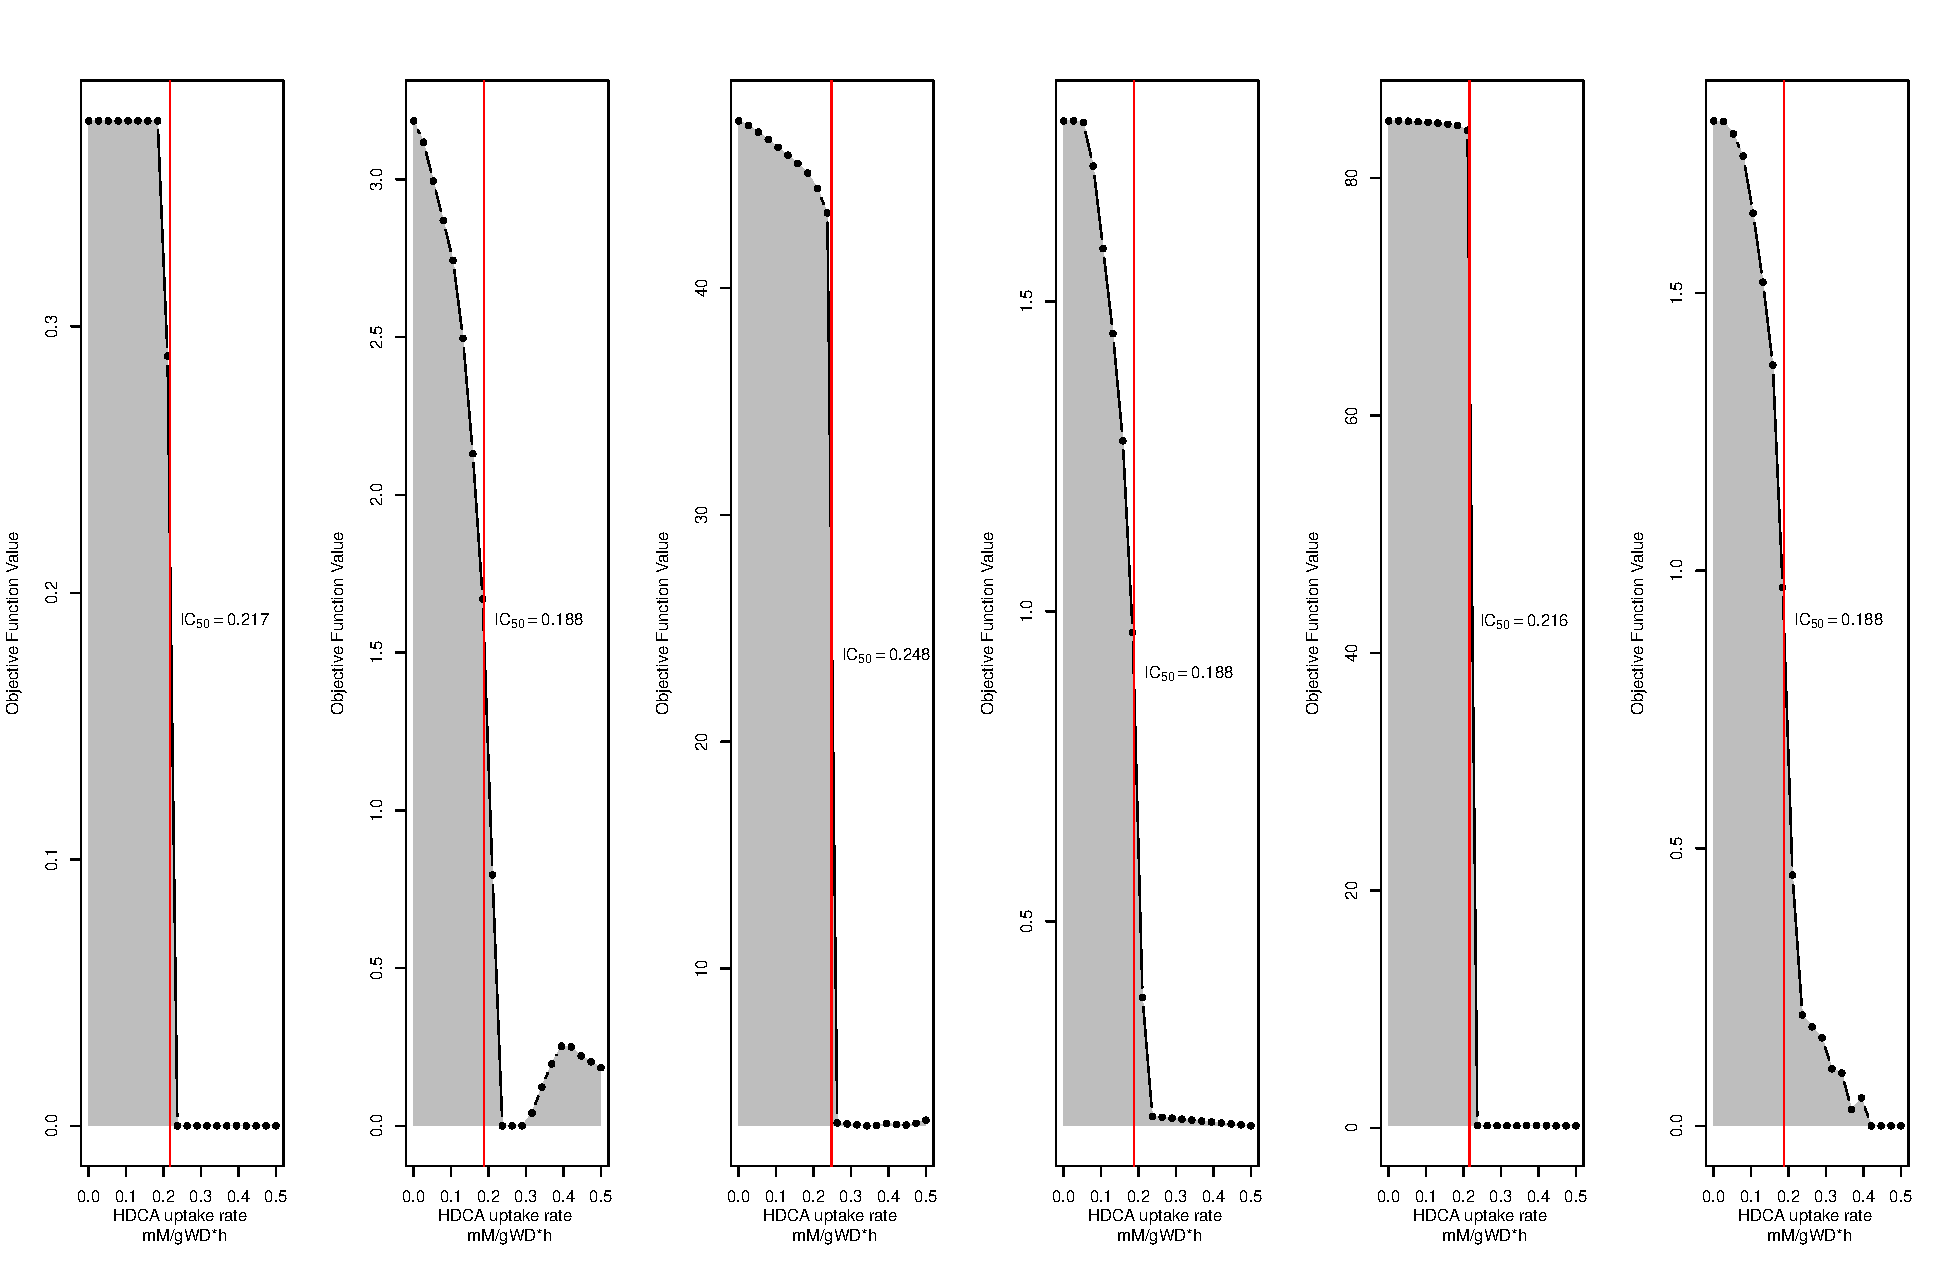
\includegraphics[width=\textwidth]{neuroprotective/IC50}
%\end{center}
%\caption{Robutness analysis to calculate IC50 value for each objective function described in table \ref{OF}. Red line represents the calculated IC50 value.}
%\end{figure}
%\begin{figure}[h]
%\begin{center}
%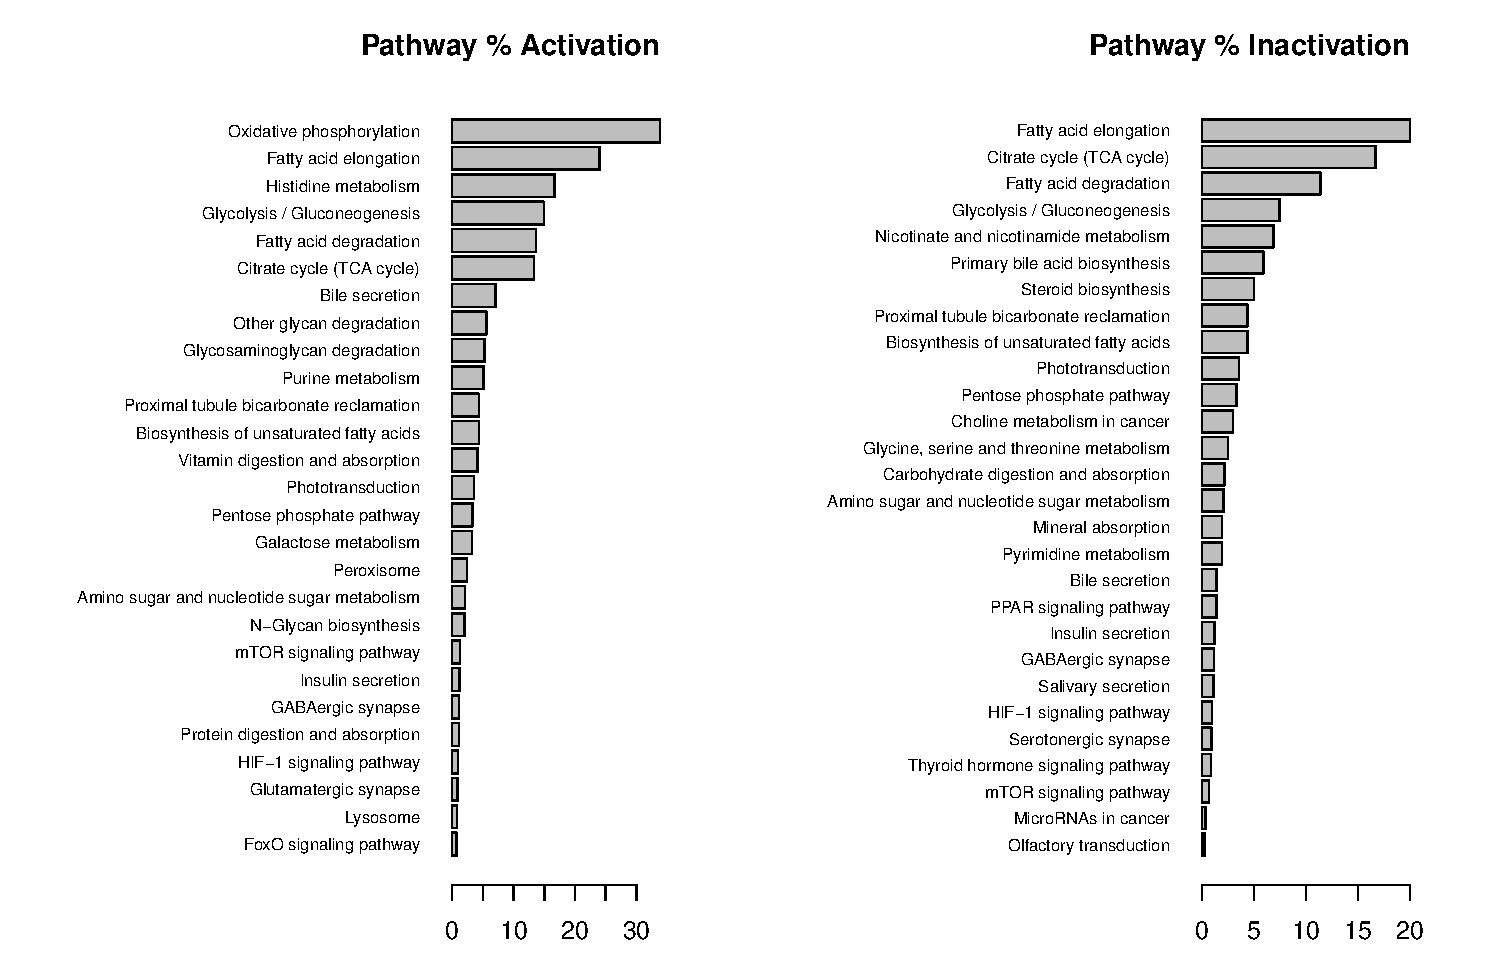
\includegraphics[width=\textwidth]{neuroprotective/Healthy2Inflammated}
%\end{center}
%\caption{Metabolic pathways affected by inflammation. Activation and inactivation percentage was measured in comparison with genes associated to each pathway in the KEGG database.}
%\end{figure}
%\begin{figure}[h]
%\begin{center}
%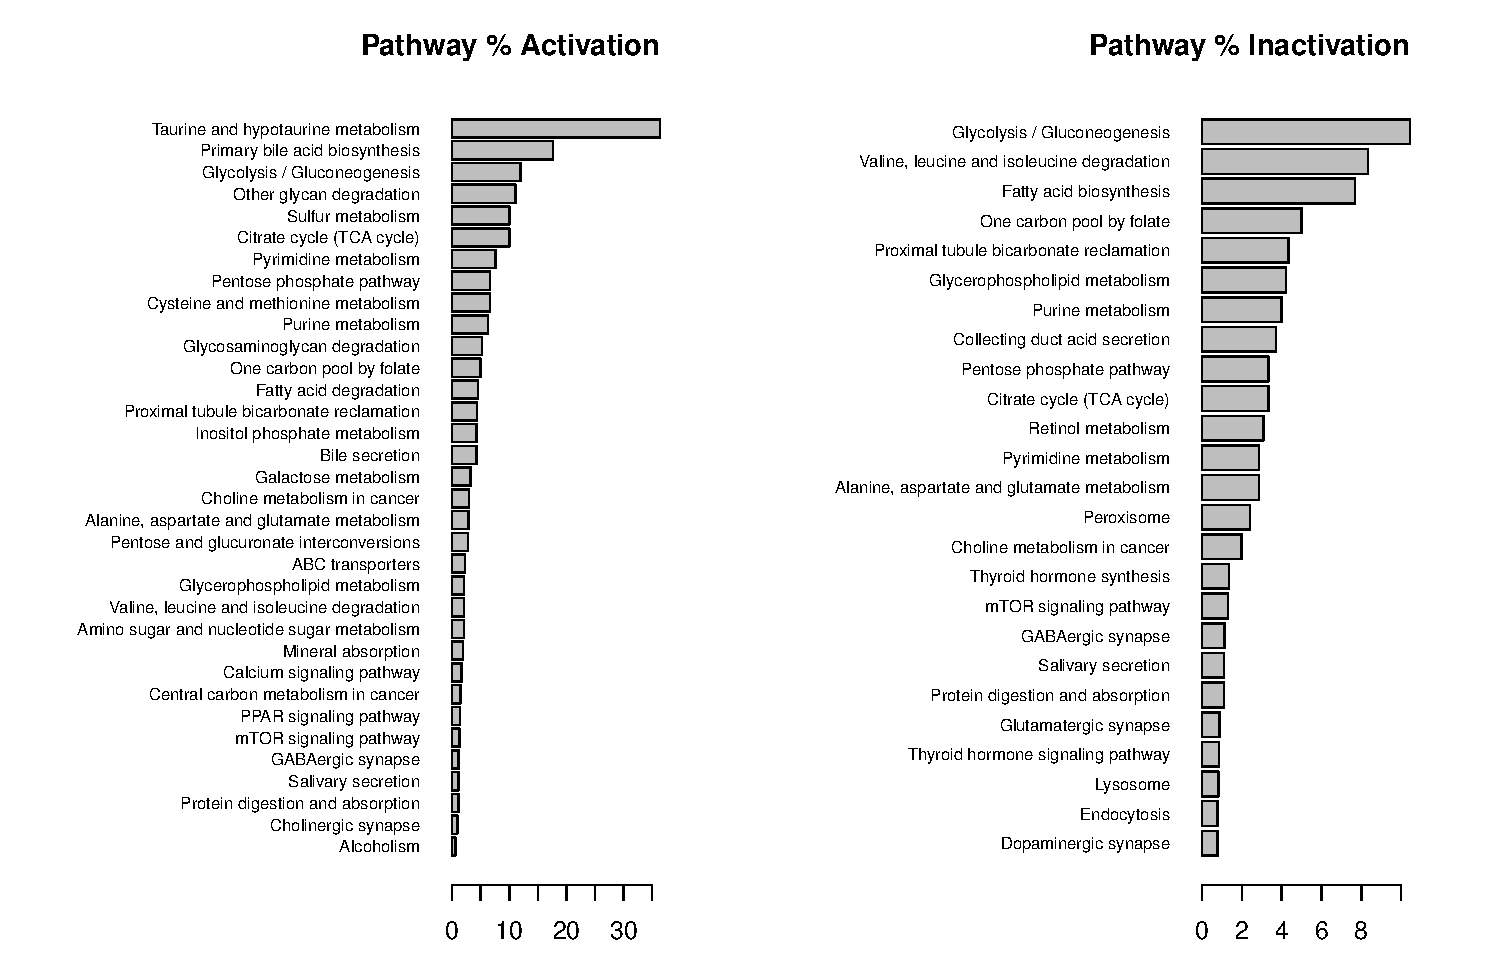
\includegraphics[width=\textwidth]{neuroprotective/Inflammated2Tibolone}
%\end{center}
%\caption{•}
%\end{figure}
\section{Conclusion}
